% !TEX root = ../diary-book.tex

\section{令和7年01月04日 Muon の一次宇宙線エネルギー依存性}

\begin{figure}
   \centering
   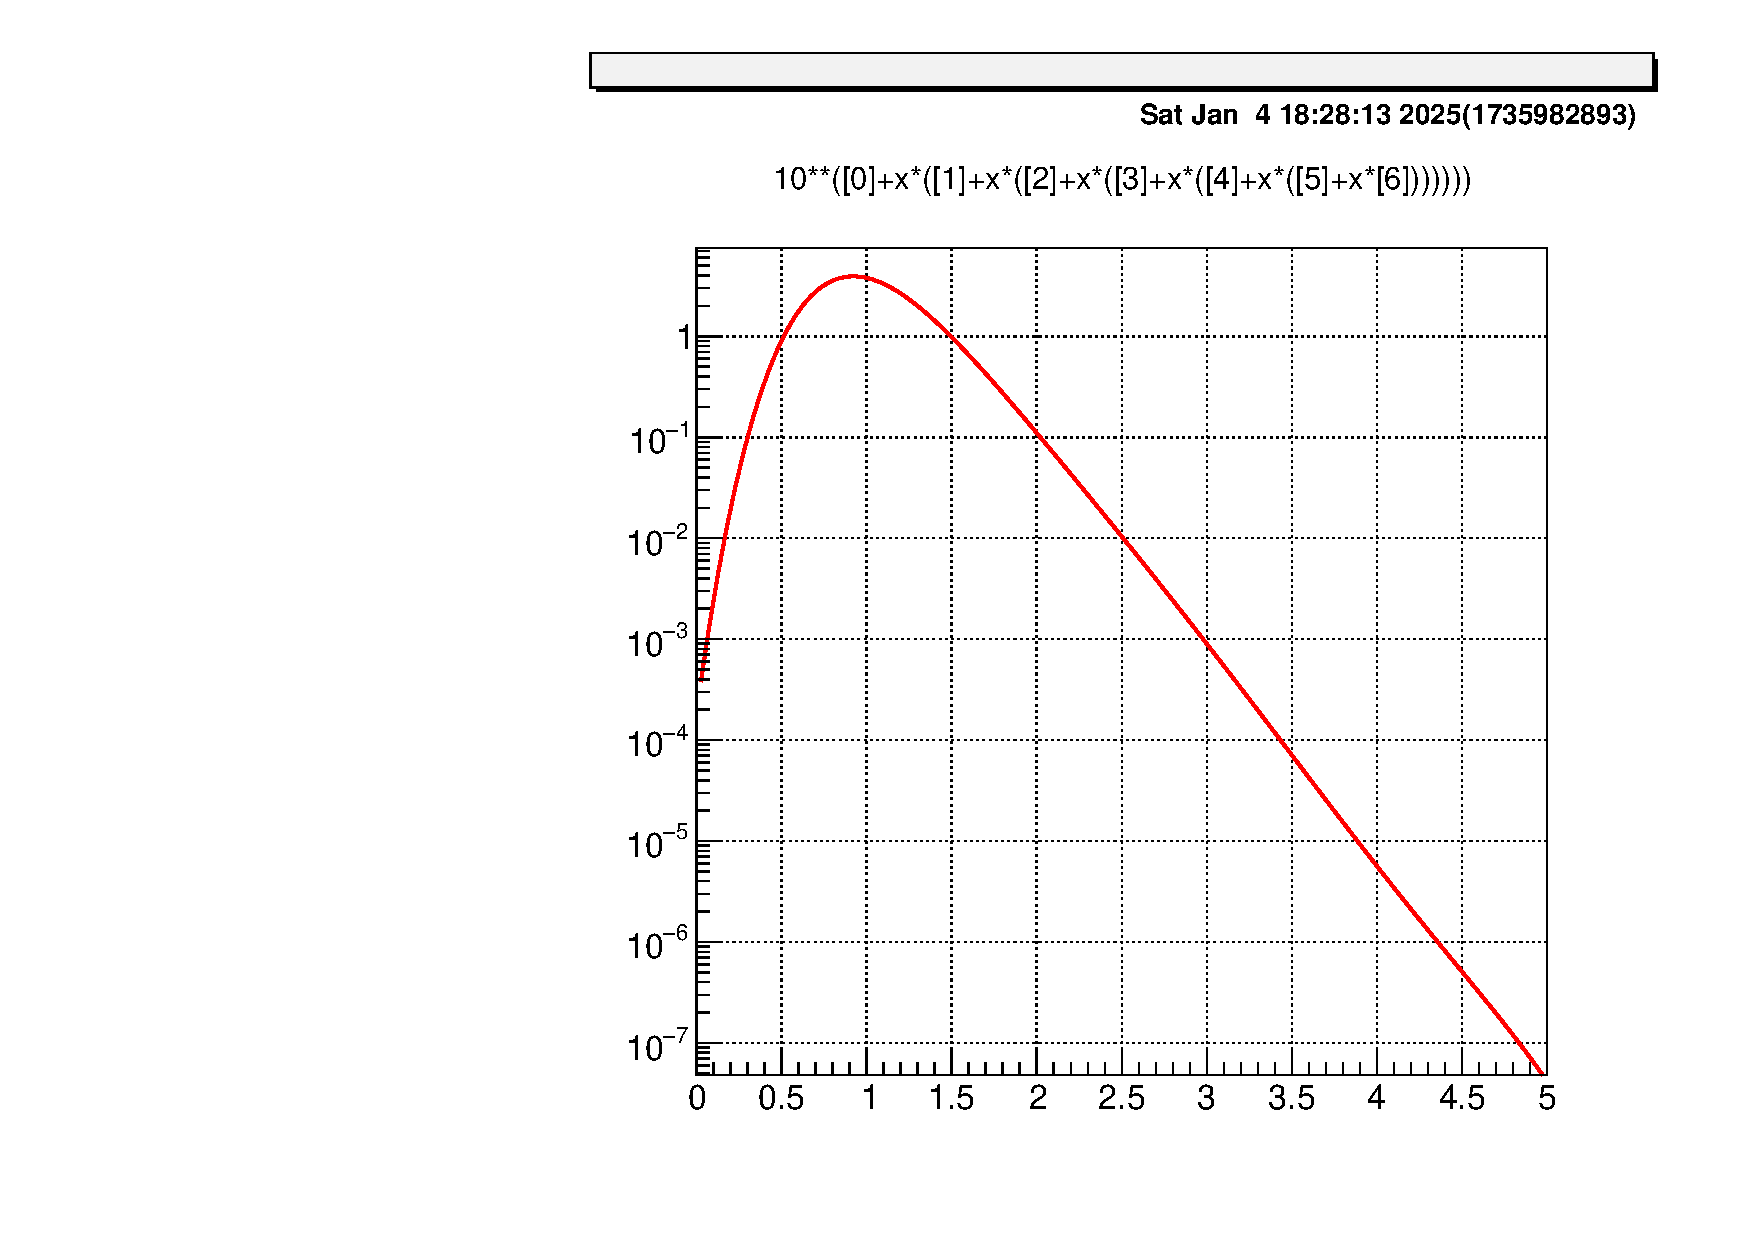
\includegraphics[width=.7\linewidth]{../../figs/ata03/figs/20250104/1735982893.pdf}
   \caption{ミュオン到来数の一次宇宙線のエネルギー依存性。横軸はエネルギーの対数、縦軸は GeV あたり、単位面積当たり、単位立体角あたりの個数。ログを取ったものに六次関数を当てはめた。}
\end{figure}


\begin{figure}
   \centering
   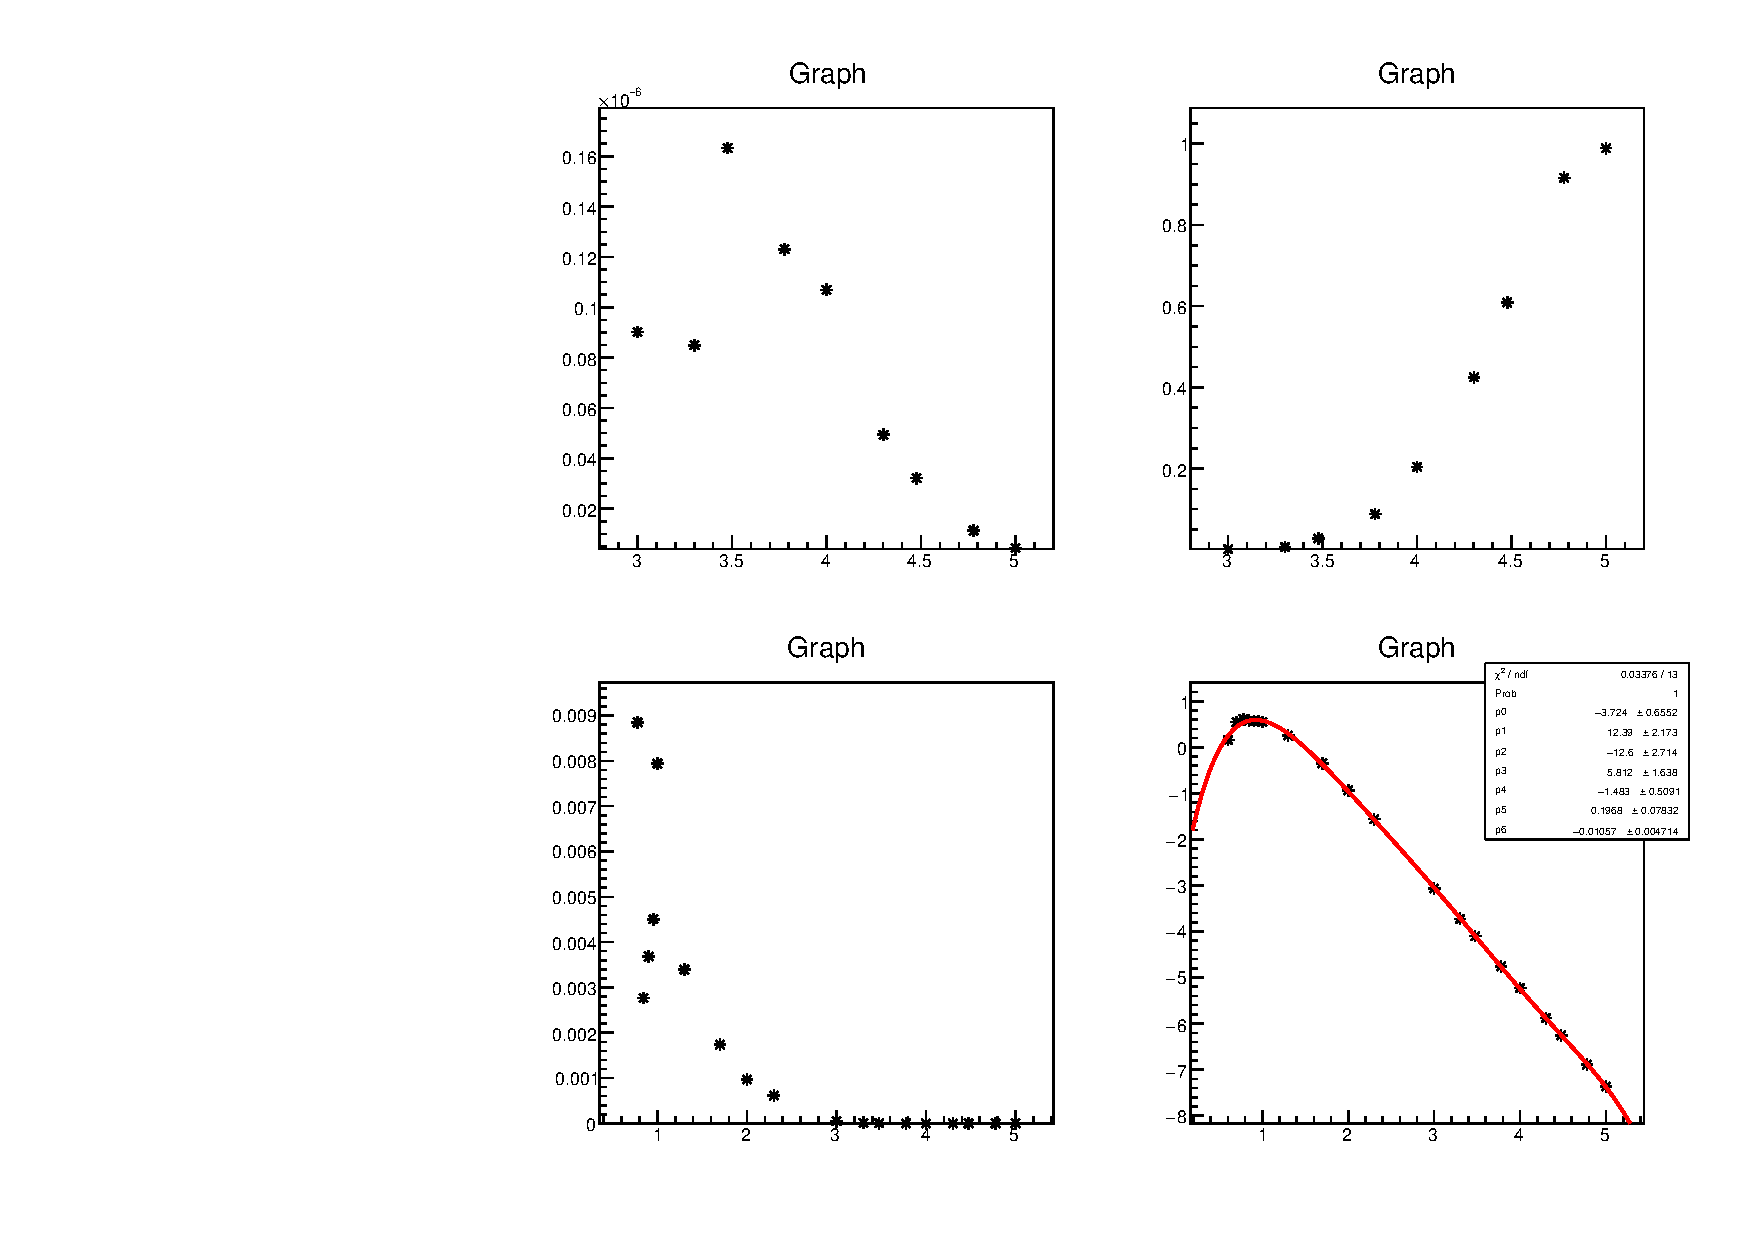
\includegraphics[width=.7\linewidth]{../../figs/ata03/figs/20250104/1735983065.pdf}
   \caption{左上：ミュオンとシャワーの同時計数、右上：シャワー面同定の効率、左下：サイトでのミュオンの計測個数、右下：ミュオンの到来数}
\end{figure}

